\newpage
\null
\thispagestyle{empty}
\newpage

\addcontentsline{toc}{chapter}{Song of Solomon}

% Safely inserts your illustration full-bleed on its own page.
% This completely bypasses the page builder, headers, and geometry bugs!
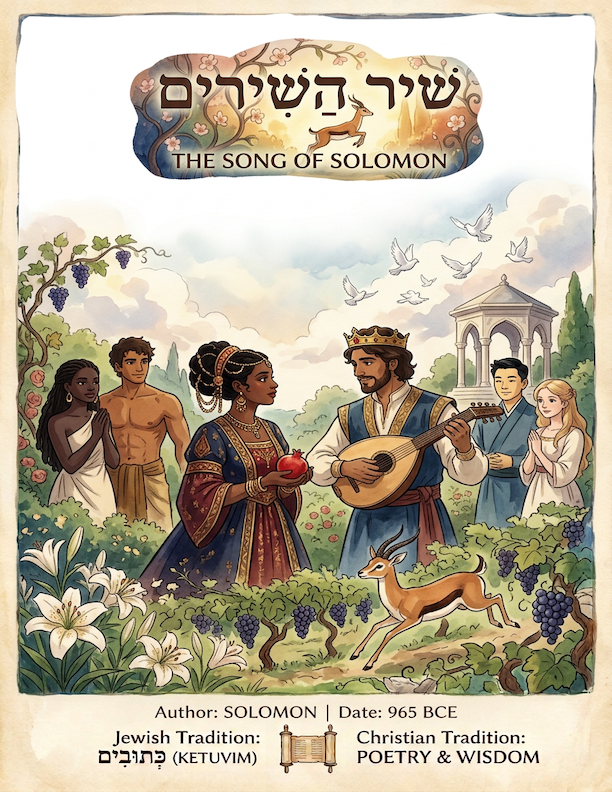
\includepdf[pages=1, fitpaper=false, width=\paperwidth, height=\paperheight, , keepaspectratio=false]{images/divider2/songofsolomon_2.png}
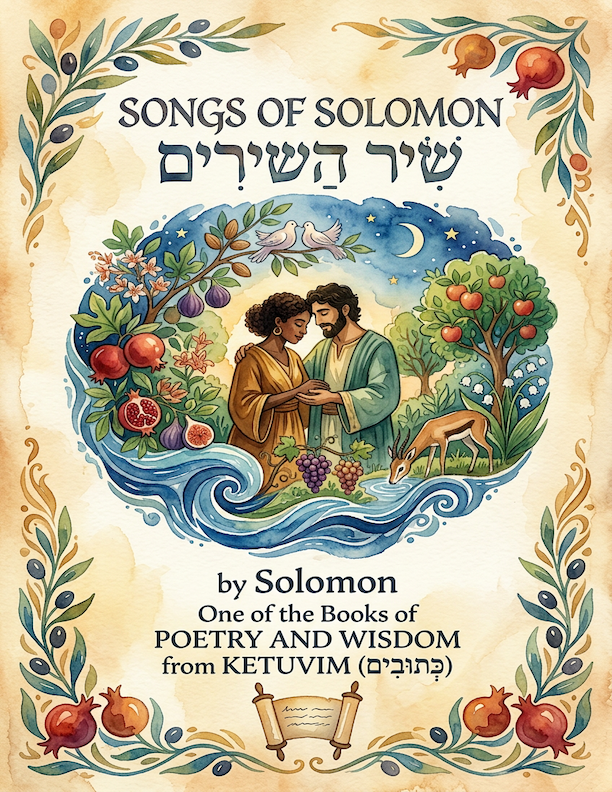
\includepdf[pages=1, fitpaper=false, width=\paperwidth, height=\paperheight, , keepaspectratio=false]{images/divider1/songofsolomon.png}
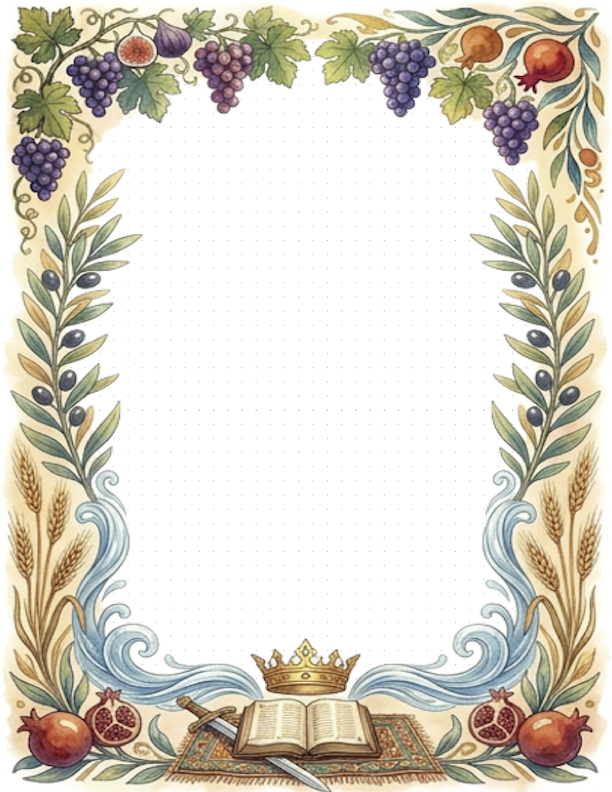
\includepdf[pages=1, fitpaper=false, width=\paperwidth, height=\paperheight, , keepaspectratio=false]{images/8.5x11-Dot-Grid.png}
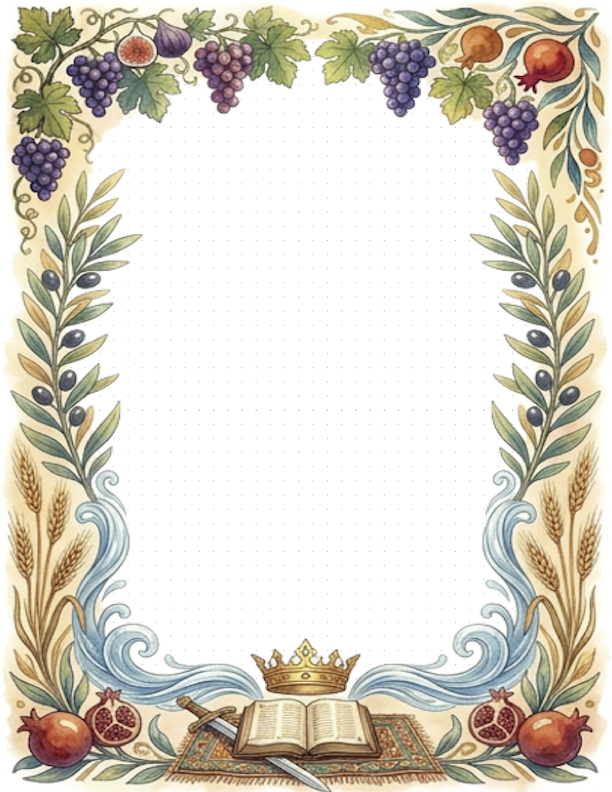
\includepdf[pages=1, fitpaper=false, width=\paperwidth, height=\paperheight, , keepaspectratio=false]{images/8.5x11-Dot-Grid.png}
\mybook{Song of Solomon}
\vspace{-1.36in}
\begin{multicols}{2}
\mychapter{} \myverse*{}The Song of songs, which is Solomon’s.


\textit{Beloved}

\myverse{}Let him kiss me with the kisses of his mouth;

for your love is better than wine.

\myverse{}Your oils have a pleasing fragrance.

Your name is oil poured out,

therefore the virgins love you.

\myverse{}Take me away with you.

Let’s hurry.

The king has brought me into his rooms.

\textit{Friends}

We will be glad and rejoice in you.

We will praise your love more than wine!

\textit{Beloved}

They are right to love you.

\myverse{}I am dark, but lovely,

you daughters of Jerusalem,

like Kedar’s tents,

like Solomon’s curtains.

\myverse{}Don’t stare at me because I am dark,

because the sun has scorched me.

My mother’s sons were angry with me.

They made me keeper of the vineyards.

I haven’t kept my own vineyard.

\myverse{}Tell me, you whom my soul loves,

where you graze your flock,

where you rest them at noon;

for why should I be as one who is veiled

beside the flocks of your companions?


\textit{Lover}

\myverse{}If you don’t know, most beautiful among women,

follow the tracks of the sheep.

Graze your young goats beside the shepherds’ tents.

\vspace{\baselineskip}

\myverse{}I have compared you, my love,

to a steed in Pharaoh’s chariots.

\myverse{}Your cheeks are beautiful with earrings,

your neck with strings of jewels.


\textit{Friends}

\myverse{}We will make you earrings of gold,

with studs of silver.


\textit{Beloved}

\myverse{}While the king sat at his table,

my perfume spread its fragrance.

\myverse{}My beloved is to me a sachet of myrrh,

that lies between my breasts.

\myverse{}My beloved is to me a cluster of henna blossoms

from the vineyards of En Gedi.


\textit{Lover}

\myverse{}Behold,\footnote{1:15 “Behold”, from “הִנֵּה”, means look at, take notice, observe, see, or gaze at. It is
	often used as an interjection.} you are beautiful, my love.

Behold, you are beautiful.

Your eyes are like doves.


\textit{Beloved}

\myverse{}Behold, you are beautiful, my beloved, yes, pleasant;

and our couch is verdant.


\textit{Lover}

\myverse{}The beams of our house are cedars.

Our rafters are firs.


%SOS 2
\mychapter{}\textit{Beloved}

\myverse*{}I am a rose of Sharon,

a lily of the valleys.


\textit{Lover}

\myverse{}As a lily among thorns,

so is my love among the daughters.


\textit{Beloved}

\myverse{}As the apple tree among the trees of the wood,

so is my beloved among the sons.

I sat down under his shadow with great delight,

his fruit was sweet to my taste.

\myverse{}He brought me to the banquet hall.

His banner over me is love.

\myverse{}Strengthen me with raisins,

refresh me with apples;

for I am faint with love.

\myverse{}His left hand is under my head.

His right hand embraces me.

\myverse{}I adjure you, daughters of Jerusalem,

by the roes, or by the hinds of the field,

that you not stir up, nor awaken love,

until it so desires.

\vspace{\baselineskip}

 \myverse{}The voice of my beloved!

Behold, he comes,

leaping on the mountains,

skipping on the hills.

\myverse{}My beloved is like a roe or a young deer.

Behold, he stands behind our wall!

He looks in at the windows.

He glances through the lattice.

\vspace{\baselineskip} 

\myverse{}My beloved spoke, and said to me,

“Rise up, my love, my beautiful one, and come away.

\myverse{}For behold, the winter is past.

The rain is over and gone.

\myverse{}The flowers appear on the earth.

The time of the singing has come,

and the voice of the turtledove is heard in our land.

\myverse{}The fig tree ripens her green figs.

The vines are in blossom.

They give out their fragrance.

Arise, my love, my beautiful one,

and come away.”


\textit{Lover}

\myverse{}My dove in the clefts of the rock,

in the hiding places of the mountainside,

let me see your face.

Let me hear your voice;

for your voice is sweet and your face is lovely.

\myverse{}Catch for us the foxes,

the little foxes that plunder the vineyards;

for our vineyards are in blossom.


\textit{Beloved}

\myverse{}My beloved is mine, and I am his.

He browses among the lilies.

\myverse{}Until the day is cool, and the shadows flee away,

turn, my beloved,

and be like a roe or a young deer on the mountains of Bether.


% SOS 3
\mychapter{} \myverse*{}By night on my bed,

I sought him whom my soul loves.

I sought him, but I didn’t find him.

\myverse{}I will get up now, and go about the city;

in the streets and in the squares I will seek him whom my soul loves.

I sought him, but I didn’t find him.

\myverse{}The watchmen who go about the city found me;

“Have you seen him whom my soul loves?”

\myverse{}I had scarcely passed from them,

when I found him whom my soul loves.

I held him, and would not let him go,

until I had brought him into my mother’s house,

into the room of her who conceived me.

\vspace{\baselineskip} 

\myverse{}I adjure you, daughters of Jerusalem,

by the roes, or by the hinds of the field,

that you not stir up nor awaken love,

until it so desires.

\vspace{\baselineskip} 

\myverse{}Who is this who comes up from the wilderness like pillars of smoke,

perfumed with myrrh and frankincense,

with all spices of the merchant?

\myverse{}Behold, it is Solomon’s carriage!

Sixty mighty men are around it,

of the mighty men of Israel.

\myverse{}They all handle the sword, and are expert in war.

Every man has his sword on his thigh,

because of fear in the night.


\vspace{\baselineskip}

 \myverse{}King Solomon made himself a carriage

of the wood of Lebanon.

\myverse{}He made its pillars of silver,

its bottom of gold, its seat of purple,

the middle of it being paved with love,

from the daughters of Jerusalem.

\myverse{}Go out, you daughters of Zion, and see King Solomon,

with the crown with which his mother has crowned him,

in the day of his weddings,

in the day of the gladness of his heart.


% SOS 4
\mychapter{}\textit{Lover}

\myverse*{}Behold, you are beautiful, my love.

Behold, you are beautiful.

Your eyes are like doves behind your veil.

Your hair is as a flock of goats,

that descend from Mount Gilead.

\myverse{}Your teeth are like a newly shorn flock,

which have come up from the washing,

where every one of them has twins.

None is bereaved among them.

\myverse{}Your lips are like scarlet thread.

Your mouth is lovely.

Your temples are like a piece of a pomegranate behind your veil.

\myverse{}Your neck is like David’s tower built for an armory,

on which a thousand shields hang,

all the shields of the mighty men.

\myverse{}Your two breasts are like two fawns

that are twins of a roe,

which feed among the lilies.


\vspace{\baselineskip}

 \myverse{}Until the day is cool, and the shadows flee away,

I will go to the mountain of myrrh,

to the hill of frankincense.


\vspace{\baselineskip} 

\myverse{}You are all beautiful, my love.

There is no spot in you.

\myverse{}Come with me from Lebanon, my bride,

with me from Lebanon.

Look from the top of Amana,

from the top of Senir and Hermon,

from the lions’ dens,

from the mountains of the leopards.


\vspace{\baselineskip}

 \myverse{}You have ravished my heart, my sister, my bride.

You have ravished my heart with one of your eyes,

with one chain of your neck.

\myverse{}How beautiful is your love, my sister, my bride!

How much better is your love than wine,

the fragrance of your perfumes than all kinds of spices!

\myverse{}Your lips, my bride, drip like the honeycomb.

Honey and milk are under your tongue.

The smell of your garments is like the smell of Lebanon.

\myverse{}My sister, my bride, is a locked up garden;

a locked up spring,

a sealed fountain.

\myverse{}Your shoots are an orchard of pomegranates, with precious fruits,

henna with spikenard plants,

\myverse{}spikenard and saffron,

calamus and cinnamon, with every kind of incense tree;

myrrh and aloes, with all the best spices,

\myverse{}a fountain of gardens,

a well of living waters,

flowing streams from Lebanon.


\textit{Beloved}

\myverse{}Awake, north wind, and come, you south!

Blow on my garden, that its spices may flow out.

Let my beloved come into his garden,

and taste his precious fruits.


% SOS 5
\mychapter{}\textit{Lover}

\myverse*{}I have come into my garden, my sister, my bride.

I have gathered my myrrh with my spice;

I have eaten my honeycomb with my honey;

I have drunk my wine with my milk.

\textit{Friends}

Eat, friends!

Drink, yes, drink abundantly, beloved.


\textit{Beloved}
\myverse{}I was asleep, but my heart was awake.

It is the voice of my beloved who knocks:

“Open to me, my sister, my love, my dove, my undefiled;

for my head is filled with dew,

and my hair with the dampness of the night.”

\myverse{}I have taken off my robe. Indeed, must I put it on?

I have washed my feet. Indeed, must I soil them?

\myverse{}My beloved thrust his hand in through the latch opening.

My heart pounded for him.

\myverse{}I rose up to open for my beloved.

My hands dripped with myrrh,

my fingers with liquid myrrh,

on the handles of the lock.

\myverse{}I opened to my beloved;

but my beloved left, and had gone away.

My heart went out when he spoke.

I looked for him, but I didn’t find him.

I called him, but he didn’t answer.

\myverse{}The watchmen who go about the city found me.

They beat me.

They bruised me.

The keepers of the walls took my cloak away from me.


\vspace{\baselineskip} \myverse{}I adjure you, daughters of Jerusalem,

If you find my beloved,

that you tell him that I am faint with love.


\textit{Friends}
\myverse{}How is your beloved better than another beloved,

you fairest among women?

How is your beloved better than another beloved,

that you do so adjure us?


\textit{Beloved}
\myverse{}My beloved is white and ruddy.

The best among ten thousand.

\myverse{}His head is like the purest gold.

His hair is bushy, black as a raven.

\myverse{}His eyes are like doves beside the water brooks,

washed with milk, mounted like jewels.

\myverse{}His cheeks are like a bed of spices with towers of perfumes.

His lips are like lilies, dropping liquid myrrh.

\myverse{}His hands are like rings of gold set with beryl.

His body is like ivory work overlaid with sapphires.

\myverse{}His legs are like pillars of marble set on sockets of fine gold.

His appearance is like Lebanon, excellent as the cedars.

\myverse{}His mouth is sweetness;

yes, he is altogether lovely.

This is my beloved, and this is my friend,

daughters of Jerusalem.


% SOS 6
\mychapter{}\textit{Friends}

\myverse*{}Where has your beloved gone, you fairest among women?

Where has your beloved turned, that we may seek him with you?


\textit{Beloved}

\myverse{}My beloved has gone down to his garden,

to the beds of spices,

to pasture his flock in the gardens, and to gather lilies.

\myverse{}I am my beloved’s, and my beloved is mine.

He browses among the lilies.


\vspace{\baselineskip} 

\textit{Lover}

\myverse{}You are beautiful, my love, as Tirzah,

lovely as Jerusalem,

awesome as an army with banners.

\myverse{}Turn away your eyes from me,

for they have overcome me.

Your hair is like a flock of goats,

that lie along the side of Gilead.

\myverse{}Your teeth are like a flock of ewes,

which have come up from the washing,

of which every one has twins;

not one is bereaved among them.

\myverse{}Your temples are like a piece of a pomegranate behind your veil.


\vspace{\baselineskip}

 \myverse{}There are sixty queens, eighty concubines,

and virgins without number.

\myverse{}My dove, my perfect one, is unique.

She is her mother’s only daughter.

She is the favorite one of her who bore her.

The daughters saw her, and called her blessed.

The queens and the concubines saw her, and they praised her.


\vspace{\baselineskip}

 \myverse{}Who is she who looks out as the morning,

beautiful as the moon,

clear as the sun,

and awesome as an army with banners?


\vspace{\baselineskip}

 \myverse{}I went down into the nut tree grove,

to see the green plants of the valley,

to see whether the vine budded,

and the pomegranates were in flower.

\myverse{}Without realizing it,

my desire set me with my royal people’s chariots.


\textit{Friends}

\myverse{}Return, return, Shulammite!

Return, return, that we may gaze at you.

\textit{Lover}

Why do you desire to gaze at the Shulammite,

as at the dance of Mahanaim?


% SOS 7
\mychapter{} \myverse*{}How beautiful are your feet in sandals, prince’s daughter!

Your rounded thighs are like jewels,

the work of the hands of a skillful workman.

\myverse{}Your body is like a round goblet,

no mixed wine is wanting.

Your waist is like a heap of wheat,

set about with lilies.

\myverse{}Your two breasts are like two fawns,

that are twins of a roe.

\myverse{}Your neck is like an ivory tower.

Your eyes are like the pools in Heshbon by the gate of Bathrabbim.

Your nose is like the tower of Lebanon which looks toward Damascus.

\myverse{}Your head on you is like Carmel.

The hair of your head like purple.

The king is held captive in its tresses.

\myverse{}How beautiful and how pleasant you are,

love, for delights!

\myverse{}This, your stature, is like a palm tree,

your breasts like its fruit.

\myverse{}I said, “I will climb up into the palm tree.

I will take hold of its fruit.”

Let your breasts be like clusters of the vine,

the smell of your breath like apples.

\myverse{}Your mouth is like the best wine,

that goes down smoothly for my beloved,

gliding through the lips of those who are asleep.


\textit{Beloved}

\myverse{}I am my beloved’s.

His desire is toward me.

\myverse{}Come, my beloved! Let’s go out into the field.

Let’s lodge in the villages.

\myverse{}Let’s go early up to the vineyards.

Let’s see whether the vine has budded,

its blossom is open,

and the pomegranates are in flower.

There I will give you my love.

\myverse{}The mandrakes produce fragrance.

At our doors are all kinds of precious fruits, new and old,

which I have stored up for you, my beloved.

% SOS 8
\mychapter{} \myverse*{}Oh that you were like my brother,

who nursed from the breasts of my mother!

If I found you outside, I would kiss you;

yes, and no one would despise me.

\myverse{}I would lead you, bringing you into the house of my mother,

who would instruct me.

I would have you drink spiced wine,

of the juice of my pomegranate.

\myverse{}His left hand would be under my head.

His right hand would embrace me.


\vspace{\baselineskip} 

\myverse{}I adjure you, daughters of Jerusalem,

that you not stir up, nor awaken love,

until it so desires.


\textit{Friends}

\myverse{}Who is this who comes up from the wilderness,

leaning on her beloved?

\vspace{\baselineskip} 

\textit{Beloved}

Under the apple tree I awakened you.

There your mother conceived you.

There she was in labor and bore you.


\vspace{\baselineskip}

 \myverse{}Set me as a seal on your heart,

as a seal on your arm;

for love is strong as death.

Jealousy is as cruel as Sheol.\footnote{8:6 Sheol is the place of the dead.
}

Its flashes are flashes of fire,

a very flame of the LORD.\footnote{8:6 When rendered in ALL CAPITAL LETTERS, “LORD” or “GOD” is the translation of God’s Proper Name}

\myverse{}Many waters can’t quench love,

neither can floods drown it.

If a man would give all the wealth of his house for love,

he would be utterly scorned.


\textit{Brothers}

\myverse{}We have a little sister.

She has no breasts.

What shall we do for our sister

in the day when she is to be spoken for?


\vspace{\baselineskip}

 \myverse{}If she is a wall,

we will build on her a turret of silver.

If she is a door,

we will enclose her with boards of cedar.


\textit{Beloved}

\myverse{}I am a wall, and my breasts like towers,

then I was in his eyes like one who found peace.

\myverse{}Solomon had a vineyard at Baal Hamon.

He leased out the vineyard to keepers.

Each was to bring a thousand shekels\footnote{8:11 A shekel is about 10 grams or about 0.35 ounces, so 1000 shekels is about 10 kilograms or about
	22 pounds.} of silver for its fruit.

\myverse{}My own vineyard is before me.

The thousand are for you, Solomon,

two hundred for those who tend its fruit.


\textit{Lover}

\myverse{}You who dwell in the gardens, with friends in attendance,

let me hear your voice!


\textit{Beloved}

\myverse{}Come away, my beloved!

Be like a gazelle or a young stag on the mountains of spices!
\end{multicols}

